\documentclass[]{article}

\usepackage{graphicx}
\usepackage{mathtools}

%opening
\title{\textbf{Master's Thesis} \\ Correct Projection Mapping on - and Interaction Techniques with - Cloth-based Deformable Surfaces}

\author{Dan-Adrian Avram}
\author{\textbf{Academic Supervisors:} Kasper Hornbaek and Esben Pedersen}
\begin{document}

\maketitle
\thispagestyle{empty}
\newpage
\begin{center}
{\LARGE \textbf{Acknowledgements}}\\
\bigskip
\bigskip
...
\end{center}

\maketitle
\thispagestyle{empty}
\newpage
\thispagestyle{empty}
\begin{abstract}

\end{abstract}

\newpage

\renewcommand{\thepage}{\roman{page}}% Roman numerals for page counter
\setcounter{page}{1}
\tableofcontents

\newpage
\listoffigures
\newpage
\listoftables 
\newpage
\renewcommand{\thepage}{\arabic{page}}% Arabic numerals for page counter
\setcounter{page}{1}
\section{Introduction}



Deformable displays allow new methods of interaction with virtual scenes, which simply are not possible on flat displays. These interactions are more immersive and feel more natural to the user as they touch, push, pull or pinch the deformable surface. The interaction with the scene can now be done in a 3D space, similarly to how we interact with objects on a daily basis, while also providing a degree of haptic feedback.

The first part of the master thesis project deals with the development of a deformable display prototype on which undistorted visuals can be projected. The distortion of visuals due to irregularities in the surface of an arbitrary-shaped object (the display surface) is the main problem that must be solved. 

\subsection{Problem Description}

One of the main challenges when dealing with deformable surfaces, is correcting the distortions which arise from the user's interaction with the display. The image must be changed(the pixels must be shifted) so that the contents still appear as on a flat surface, even when the surface becomes an arbitrary 2.5D object.

If, for example, we are sculpting into or pulling out of a piece of cloth on which visuals are projected, some degree of distortion will appear on the final image. 
The image should be undistorted in the sense that, the visuals would still look like a fixed display (rather than being deformed with the display), after the previously mentioned pull or pinch gesture is performed. The solution will involve tracking of the cloth material and the modeling of a 3D representation of the material that is deformed based on depth sensor data.

In order to solve the problem we need to first setup a scenario where one can test how images are deformed when interacting with deformable displays. In order to do this we need: a surface that can be deformed by a user(e.g.: a cloth material) which serves as our display, a projector that is used to display contents to the end user and a depth camera that is used to track the display and surface and detect changes.

\subsection{Hardware Setup}

The deformable display prototype(see figure \ref{fig:hardware_setup}) consists of the following components:
\begin{itemize}
\item Cloth display (that can be deformed) + frame
\item Projector that is used to display the visuals onto the cloth surface
\item Depth camera that is used to retrieve the cloth display’s depth information
\end{itemize}

\begin{figure}[hbtp]
    \centering
    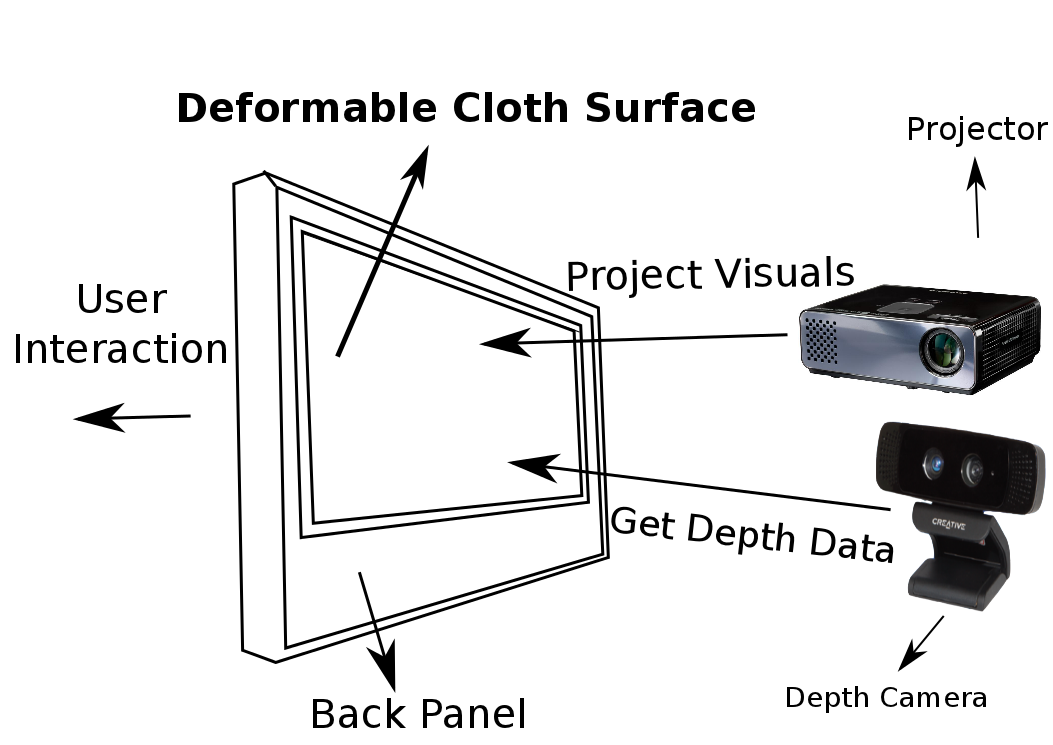
\includegraphics[width=0.8\textwidth]{figures/thesis_setup_illustration_ui.png}
    \caption{Physical setup of the prototype}
    \label{fig:hardware_setup}
\end{figure}

\section{Related Work}

In this chapter, relevant research and related works are highlighted, mainly in relation to deformable user interfaces, tracking and projection techniques on deformable surfaces, interaction techniques with deformable displays, 3D projection and the design of affordances in order to convey information or suggest particular interaction methods. Investigating related research will help in finding solutions to projection issues with deformable surfaces. Moreover, this will also be useful in order to analyze, compare and contrast different approaches to tracking as well as correcting the projection distortion. Further, existing research on interaction techniques and affordances with deformable surfaces will provide a starting point to test, design and implement relevant interaction scenarios for the prototype. Finally, work related to stereoscopic and autostereoscopic projections will be consulted, in order to arrive at a sensible projection technique that can be used in the present case.

\subsection{Tracking and Projection on Deformable Surfaces}

In this section, literature related to projections on deformable surfaces as well as possible distortion correction and tracking techniques techniques will be presented.\\

As a starting point, it makes sense to consider existing approaches of projection onto complex or non-planar physical shapes. As discussed in \cite{daalsgard11}, calibration is needed in order to correct distortions arising from a difference between the digital and the physical object. The study deals with projection on several physical objects, including a complex, organic, non-planar shape, \textbf{Holger the Dane}, as shown in figure \ref{fig:holger}.

\begin{figure}[hbtp]
    \centering
    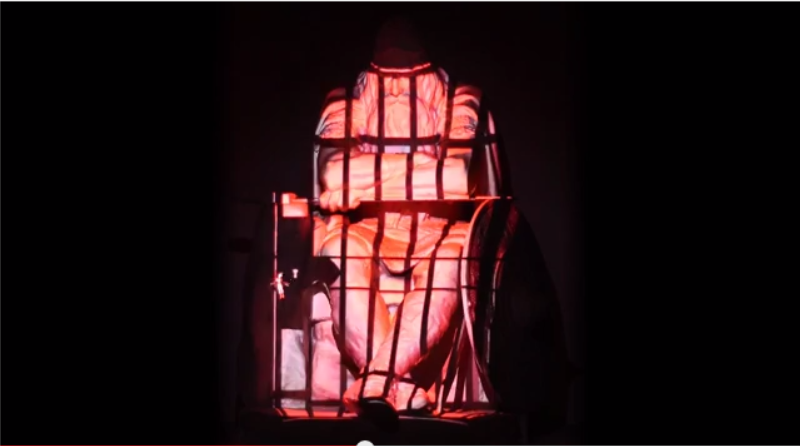
\includegraphics[width=0.8\textwidth]{figures/HolgerTheDane.PNG}
    \caption{Projection on Holger the Dane. Courtesy of \cite{daalsgard11}}
    \label{fig:holger}
\end{figure}

Further, it also proposes a few design themes for 3D projection on physical objects:
\begin{itemize}
\item New potentials for well-known 3D effects (lightning, particle systems, shadows, sound etc…).
\item Dynamics between the digital and physical world and switching between 2D and 3D projections allow to focus the projection on hotspots, while customizing properties allows outlines and switching material textures.
\item Relations between object, content and context.
\end{itemize}

Although the information about the necessity of device calibration as well as the projection on a complex surface provide some insights into the projection distortion issue at hand, the study was only concerned with projection on static objects and thus, does not address problems arising from dynamic surface deformation, where the projection would need to be adapted in real-time according to the deformable surface's depth information.\\

\textbf{FlexPad}(figure \ref{fig:flexpad}) is a real-time interactive system with a highly deformable hand-held paper display. A projector is used to display the visuals, while tracking the display surface with a depth camera provides the required depth information for detecting changes in the surface. Further, as described in \cite{steimle13}, any 2D image from Microsoft Windows can be projected and correctly warped unto the display. 


\begin{figure}[hbtp]
    \centering
    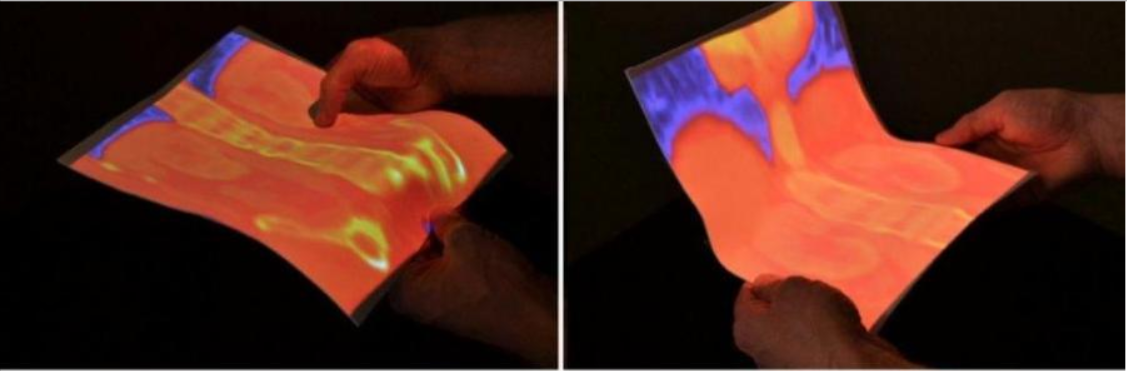
\includegraphics[width=0.8\textwidth]{figures/Flexpad.PNG}
    \caption{Interaction with Flexpad. Courtesy of \cite{steimle13}}
    \label{fig:flexpad}
\end{figure}

Moreover, a deformation model(figure \ref{fig:flexpad_deformation}) is described, in their case using a 25 x 25 vertex plane at the size of the surface. The model can be represented by a 15 dimensional vector consisting of the angles of 8 basic deformations, a z mapping parameter as well as 6 variables for DOF (degrees of freedom) required for affine 3D transformations. 

\begin{figure}[hbtp]
    \centering
    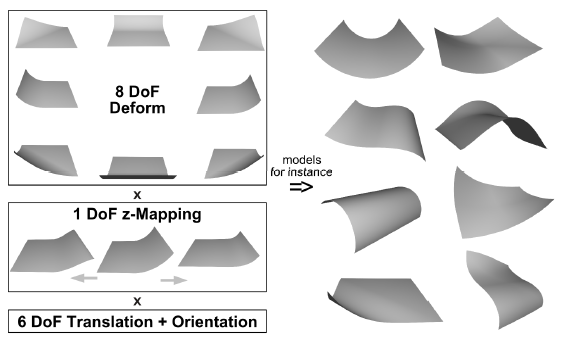
\includegraphics[width=0.8\textwidth]{figures/FlexpadDeformationModel.PNG}
    \caption{Deformation model of Flexpad(left) and deformations it can express(right). Courtesy of \cite{steimle13}}
    \label{fig:flexpad_deformation}
\end{figure}


After obtaining a deformation model, the tracking problem can be defined as finding parameters of the model such that, when synthesized as a depth image, they match the input depth image best(Analysis by Synthesis or AbS). This represents an optimization problem of finding the best parameter vector. The CMA-ES optimization scheme is used because it is a global optimization algorithm and it applies a smart distribution scheme, minimizing function evaluations needed to find an optimum. More information about these tracking methods will be presented below.

The primary limitations of the FlexPad come from those of the Kinect depth camera not being able to track very sharp bends, however these limitations could be overcome by installing several depth sensors or a more powerful sensor. The hand occlusion issue is not particularly relevant to the current project, since the depth camera will be installed in the back of the display, while interaction shall be from the front  - thus completely removing this problem.

As discussed in \cite{jordt12}, the deformation model can use NURBS surfaces, which can be easily handled via 3D control points, while being able to approximate every surface with arbitrary accuracy. These are widely used in computer graphics and can reduce the high dimensional space of all possible triangle mesh deformations.

The first step is to create an arbitrary NURBS surface using control points and knot vectors, using the algorithm discussed in \cite{jordt12}. Next, once we have a triangle mesh(which can be supplied from a modeling program or computed via OpenGL), we can approximate the mesh with a NURBS surface. The NURBS functions must be fitted to the mesh by minimizing the distance between the surface face function and the vertices of the mesh, or, in other words, finding control points for a given set of vertices, that minimize the sum over all squared distances. Mesh registration can then be performed by associating each 3D vertex coordinates to the previously generated NURBS surface. After this step, the mesh can be translated, rotated and deformed by displacing the control points of the NURBS surface function. Now we can apply an AbS method with a CMA-ES optimization scheme.\\

\textbf{DeforMe} is a projection-based mixed reality (MR) technique, which provides a method for augmenting deformable surfaces with deformation rendering graphics, as described in [4]. Projected graphics are realistically deformed to match the deformed surfaces. Mixed reality creates the illusion of a virtual modification of the physical surfaces. In this study, a flexible surface is used to allow the user to interact with the projected graphics while obtaining tactile feedback. Further, they present some drawbacks of existing tracking methods such as measuring surface deformation via a depth camera, which is not applicable to tangential deformations that can appear on a surface in a horizontal direction during interactions (e.g.: touching, pulling, etc.). To summarize, DeforMe is a projection-based MR system which allows projected graphics to be deformed to the deformation of the real object, while performing real-time estimations of the tangential deformation flows with a small number of feature points. Various deformable materials can be used without prior knowledge of their mechanical properties or deformation models. However, since depth information can be measured for a cloth-based deformable display (with the material properties being known), it is unclear if there is an immediate advantage of this method, for the current project, over the tracking techniques employed in the FlexPad system.\\

Another project that provides useful information on projecting onto irregular 3D surfaces, as well as tracking them using depth data, is \textbf{The Office of the Future}(see \cite{raskar98}). One of their objectives is to use real surfaces in the office, as spatially immersive display surfaces. High-resolution graphics is projected onto these surfaces(see figure \ref{fig:future_office}).

\begin{figure}[hbtp]
    \centering
    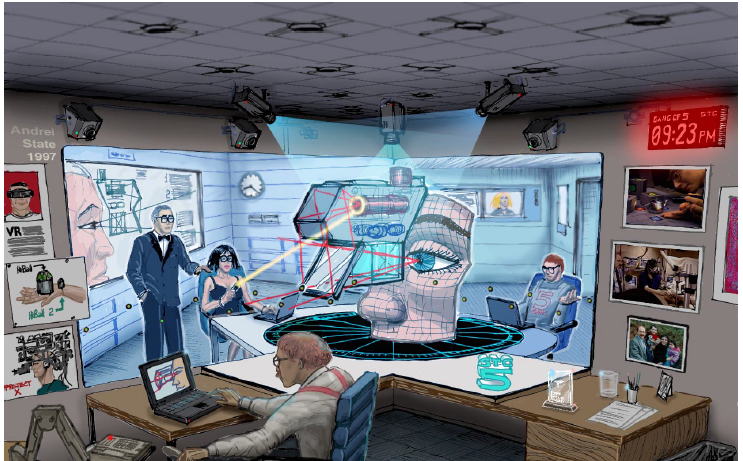
\includegraphics[width=0.8\textwidth]{figures/FutureOffice.PNG}
    \caption{The Future Office. Courtesy of \cite{raskar98}}
    \label{fig:future_office}
\end{figure}

They extract depth using imperceptible structured light (projecting binary-coded patterns that are not detected by the visible eye and recording the images with video cameras) - this process can be replaced in the current project by the use of an off-the-shelf depth camera. Further, they describe how, by knowing the object's surface, the viewer's location, projector calibration parameters and the contents to be projected, they can render on irregular 3D surfaces by the use of conventional 3-D methods(e.g.: projective texture mapping), in real-time. Finally, they state that their system can be used to detect display surface changes at non-interactive rates. However, due to a large increase in computing power in recent years, and the possibility to write graphics programs that run directly on the hardware(e.g.: shader programs), similar techniques can be used today, to detect display surface changes in real-time.\\

\textbf{The Deformable Workspace}(see figure \ref{fig:deformable_workspace}) is another approach to creating a deformable screen that acts as a boundary surface between the real and virtual worlds and is presented in [5]. The workspace is set up in similar ways to other techniques by using an IR camera, IR projector and an LCD projector. Basically, the IR camera and projector could be replaced by a depth sensor such as the Kinect. 

\begin{figure}[hbtp]
    \centering
    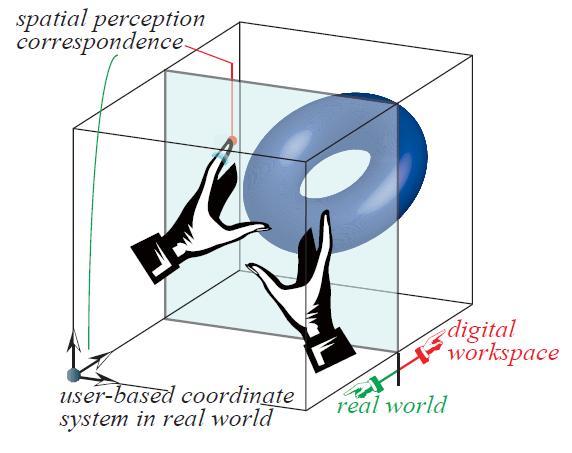
\includegraphics[width=0.8\textwidth]{figures/TheDeformableWorkspace.PNG}
    \caption{The Deformable Workspace Setup. Courtesy of \cite{watanabe08}}
    \label{fig:deformable_workspace}
\end{figure}

Tracking is based on triangulation using structured light. A single snapshot of the illuminated surfaces is sufficient to grasp complete screen deformation - a high-speed camera acquires the image, and a dedicated co-processor for high-speed image processing calculates the coordinates of a 3D point for each spot of light in the pattern (real-time performance at 955fps with a latency of 4.5ms), as described in \cite{watanabe07}. Although the frame rate achieved is incredibly high, this is a custom solution, that requires separate hardware. The previous method shall not be employed for this project as the deformable display can now be tracked with a standard depth camera(either a structured light or time-of-flight depth camera).

In [5] they also provide a method to compensate for projection distortion, given that both the calibration parameters and the shape of the deformed screen are known. An observation model in human vision is required to solve this issue, in this case, perspective projection. The technique involves pre-warping the image by shifting each projected point. Further, they claim that projective texture mapping can be used to calculate and render the warped image to be projected in real-time, efficiently and easily. A limitation of the previous approach is that an assumption has been made that the user’s eyes are fixed. However, a viewpoint-based projection should be employed to accommodate realistic scenarios - the virtual space must be rotated and transformed according to the change of viewpoint.\\

As a final note, we can observe that the techniques used to project onto irregular objects and of correcting the visuals are similar in \cite{watanabe08} and \cite{raskar98}: both extract depth information and form a polygonal model of the target object, they use the same rendering technique(projective texture mapping) and require the same calibration parameters. 

\subsection{Interaction Techniques with Deformable Surfaces}

\section{Prototype Design}

Both the projector and the depth camera will be fixed in place relative to the deformable screen. Further, the projected visuals will be interactive applications that need to be rendered continuously. Finally, due to the fact that the projected image will be warped (distorted) according to the screen deformation, an algorithm is needed to shift the projected image pixels corresponding to the display surface’s depth data. 

\begin{figure}[hbtp]
    \centering
    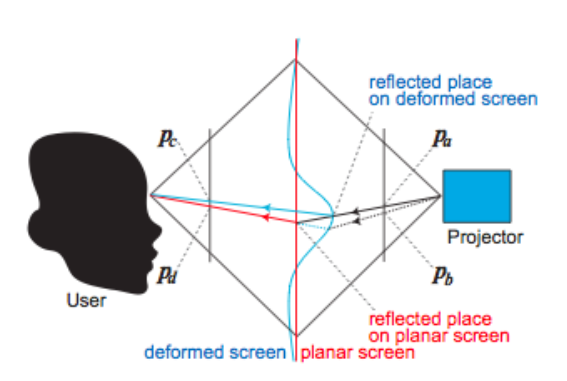
\includegraphics[width=0.8\textwidth]{figures/PointProjection.PNG}
    \caption{Compensation of image warp caused by screen deformation. Courtesy of \cite{watanabe08}}
    \label{fig:PointCompensation}
\end{figure}

In figure \ref{fig:PointCompensation}, $p_{d}$ is the position where the ray is observed for a planar screen, while $p_{c}$ is that of the deformed screen, if the projection is from $p_{a}$. To observe $p_{d}$ for the deformed screen, projection must be from point $p_{b}$. Consequently, the image point needs to be translated to this position, in order to compensate for the distortion.\\

A possible approach to solving the distortion issue is discussed in \cite{watanabe08}, where the authors state that in order to compensate for the distortions of the display one needs to know the shape of the deformed screen (depth data) and the projector calibration parameters. \\

Perhaps another solution would be to use some kind of spatial distortion, similar to the approach used for the \textbf{JellyLens} (see \cite{pindat12}). The focus + context lens(uses two levels of detail to connect a magnified region to the selected context)  can dynamically adapt to the shape of the objects of interest. As we can see in figure  \ref{fig:JellyLens}, the object of interest adapts its shape(is magnified), while the context is preserved - surrounding objects are almost untouched by the applied distortion.

\begin{figure}[hbtp]
    \centering
    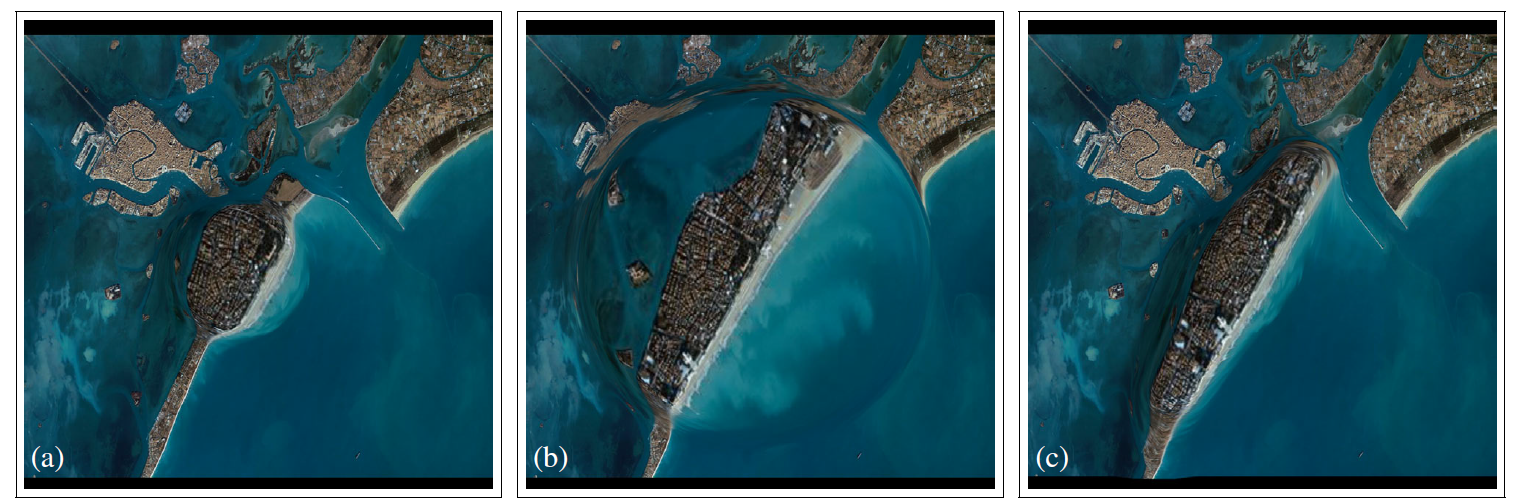
\includegraphics[width=0.8\textwidth]{figures/JellyLens.PNG}
    \caption{a) Only a portion of the object can be magnified with a small fisheye lens; b) A large fisheye magnifies almost the entire object, but at the cost of added distortion for sorrounding objects; c) JellyLens - adapting the relevant information of the object, while preserving the surrounding areas. Courtesy of \cite{pindat12}}
    \label{fig:JellyLens}
\end{figure}

The JellyLens can adapt to match the geometry in a three-step process:
\begin{itemize}
\item Obtaining information about the geometry of the objects (in our case, this can be accomplished by transforming our object depth data to 3D geometry)
\item Computing the lens shape according to its position and visualization and to the geometry of the nearby objects of interest (in our case, the depth data can be used to determine how to shape the lens)
\item Rendering of the region seen through the lens (in our case, we can apply a normal texture on the deformable mesh's geometry - that represents the contents, and distort it according to the lens shape obtained previously)
\end{itemize}

The authors of \cite{pindat12} also describe in detail how to model and adapt the lens using two techniques known as \textit{AreaLens} and \textit{PathLens}. For more detail about the process, please consult this reference.\\

For this project, a solution similar to that employed in \cite{watanabe08} has been implemented. In order to get a better overview and understanding of the whole process required to correct the distortions, I have created a system pipeline(see figure \ref{fig:Pipeline}) that describes the whole process, at a high-level. Each part will be described individually in subsequent chapters.

\begin{figure}[hbtp]
    \centering
    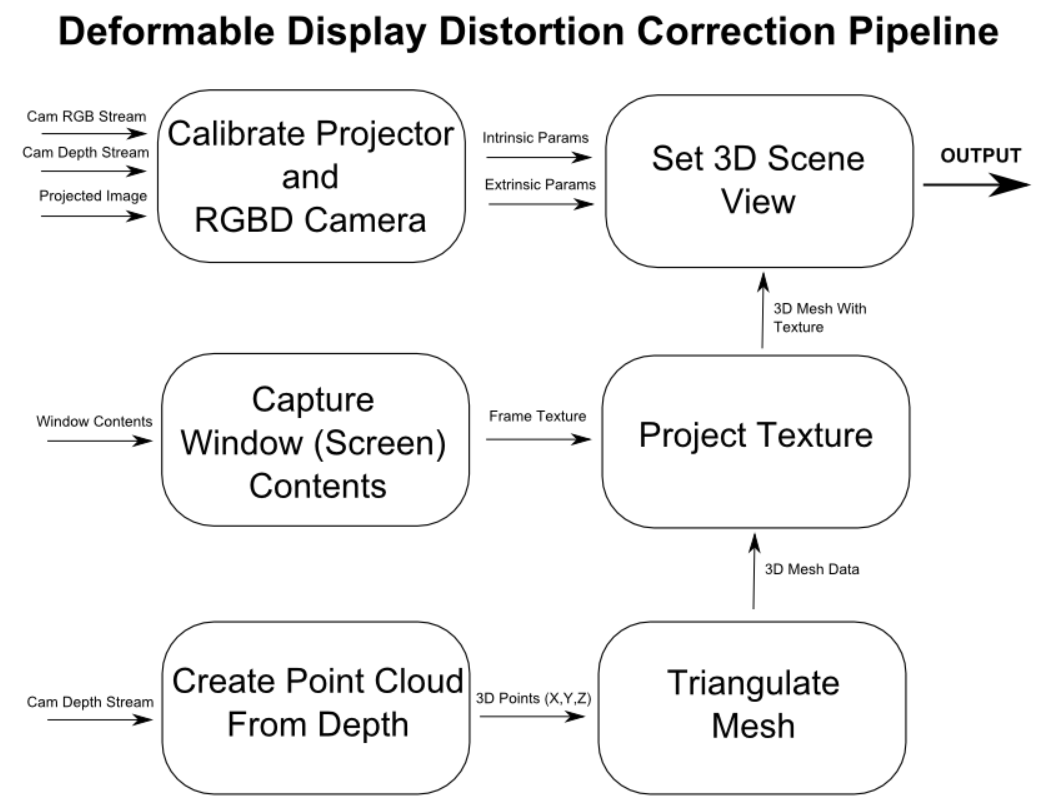
\includegraphics[width=0.8\textwidth]{figures/DeformableDisplayPipeline.PNG}
    \caption{Distortion Correction Pipeline}
    \label{fig:Pipeline}
\end{figure}

\section{Prototype Development}

Considering our system pipeline, I will explain briefly, how the whole components work and why they are needed, in this section. The first process is calibration. Note that the order in which components are explained does not represent the flow in the pipeline, since it will be easier to see, for example, why calibration is needed once some of the other steps have been explained.\\

The idea followed in \cite{watanabe08} consists of displaying the final application contents on a 3D model representation of the deformable surface. In order to obtain a relatively stable model, one can convert the depth data into a 3D mesh. An intermediary step required in order to do so, is to first create a point cloud from the depth data, or in other words, to use the depth value as the z-coordinate and create a cloud of points with coordinates $(X, Y, Z)$ corresponding to the image pixels and depth.\\

Further, the application contents must be displayed in such a way that they distort with the object. Like with most problems in computer graphics, there is more than one solution. One could, for example, use raytracing to directly project rays of light on the object(also mentioned by the authors of \cite{raskar98}. However, this approach is known to be slow and may not run in real-time. Alternatively, there exists a technique which has been tried and tested before, known in computer graphics, which projects a texture onto an object as from a slide projector. This technique can also be implemented in real-time on modern hardware, and, since the texture is projected from a virtual projector in the 3D scene, it will update with the distortions corresponding to the deformation on the object.\\

Finally, we need to make sure that our virtual camera corresponds, as closely as possible to the area we project onto with our physical display. Further, we also need to place our virtual projector, which also requires information about where the mesh(3D model) is placed, and how it is oriented. In addition to position and orientation we must also know the field of view(FOV), or the \textit{"zoom level"} of our camera(as the other parameters depend on the FOV). In addition to the calibration required above, one also needs to manually(physically) align the projector so that if correctly fills the deformable display area. Furthermore, in case of manual calibration, the depth camera must also be placed as orthogonal as possible to the deformable surface area, so that it is easy to obtain acceptable parameters for the virtual camera and projector described above. 

At this point, we basically have a solution to the distortion correction problem. The only remaining issue is to update the application contents dynamically, by capturing window/screen contents. This can be accomplished by using textures.

In the next sections, each of the above will be described in greater detail.

\subsection{Calibration of the Projector and the Depth Camera}

In order to properly display the contents on the deformable surface, three things must be ensured:
\begin{itemize}
\item The projector must be calibrated in order to find the intrinsic and extrinsic parameters that will be used to compute a transformation matrix that defines the world view of the 3D scene
\item The physical projector must be aligned with the deformable screen area. Further, the depth stream must be adjusted manually so that the deformable display is almost perfectly in view, if the calibration is done manually, by trial and error; 
\item The projector and camera are static and must not be moved, otherwise the calibration process has to be repeated\\
\end{itemize}

The calibration problem is a projector-camera calibration problem, similar to the illustration shown in figure \ref{fig:ProjectorCameraSetup}. The only difference being that, for this project, an RGBD camera(RGB stream + depth stream) is used. This means that there are two cameras: a normal RGB video camera, and a depth camera. If the calibration is done between the RGB camera and the projector, the RGB camera must then be correctly mapped to the depth camera or vice-versa.

\begin{figure}[hbtp]
    \centering
    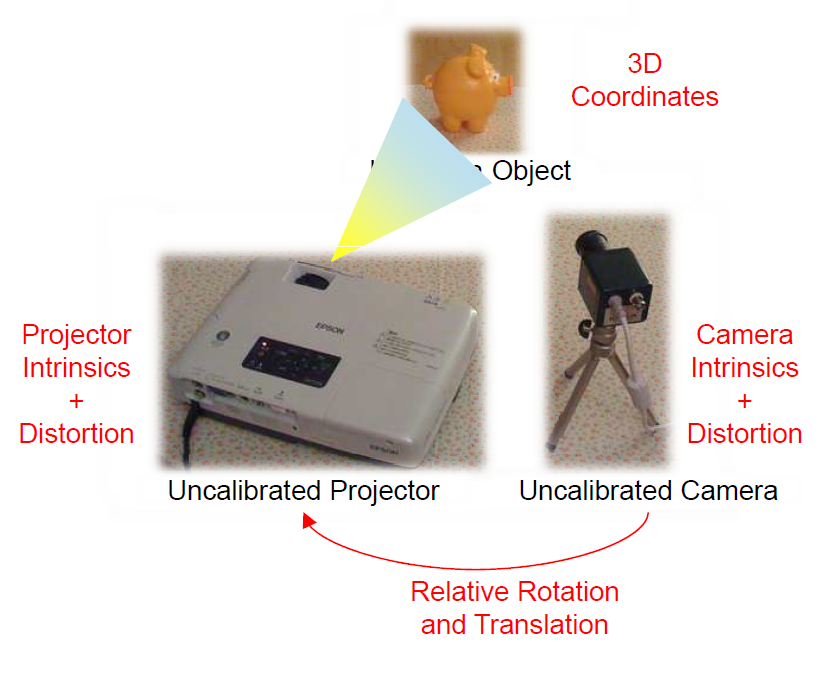
\includegraphics[width=0.8\textwidth]{figures/Projector-Camera_Calibration.PNG}
    \caption{A setup that needs projector-camera calibration}
    \label{fig:ProjectorCameraSetup}
\end{figure}

In order to properly align the physical projector/camera with the virtual projector/camera we need to compute two matrices in a virtual world, based on parameters extracted from the calibration procedure. The first is the projection matrix, which can be represented as a frustum(see figure \ref{fig:Frustum}). We can define the projection matrix in OpenGL either by providing all the frustum parameters(the near and far parameters can be entered manually), or a field of view and aspect ratio, from which they can be computed. 
\begin{figure}[hbtp]
    \centering
    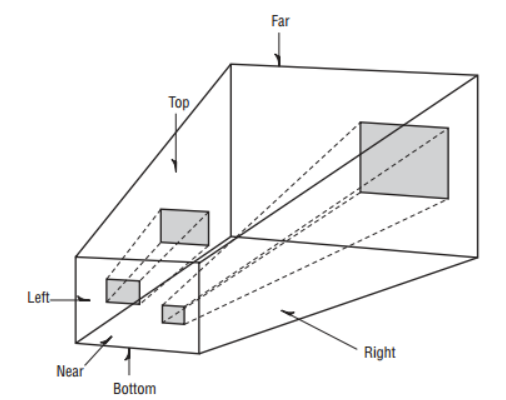
\includegraphics[width=0.8\textwidth]{figures/Frustum.PNG}
    \caption{The projection frustum. Courtesy of \cite{superbible}}
    \label{fig:Frustum}
\end{figure}

It essentially defines the viewing volume of our 3D scene. In order to compute this matrix, one needs to know the intrinsic parameters of the physical projector.
\textbf{Intrinsic parameters} refer to different aspects of a camera/projector such as focal length, scale parameters, a tilt compensation parameter and the image coordinates which define the image center or principal point. In addition, other parameters can be included to account for lens distortion. Lens distortion will not be addressed in the current project. The images projected with a modern device have low distortion.\\

Secondly, we need to compute the modelview matrix(see figure \ref{fig:MVMatrix}, for the structure of such a matrix). This matrix has information that relates to the position of the model(3D object space) as well as the camera(eye space). In this case, we essentially need to compute the view matrix from the extrinsic parameters, so that our virtual camera correctly points to the deformable display area on which our target contents are projected. \textbf{Extrinsic parameters} represent the \textbf{location} and the \textbf{orientation} of the projector/camera with respect to a world reference frame. For example, if we choose the world origin to be the position of the depth camera, then we can compute the rotation and translation of the projector with respect to the depth camera by finding the rotation matrix R and translation coefficients T. To obtain camera coordinates from world coordinates we simply need to multiply a position by R and add the translation T.

\begin{figure}[hbtp]
    \centering
    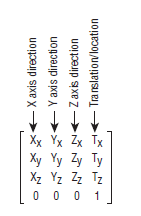
\includegraphics[width=0.4\textwidth]{figures/MVMatrixOGLSB.PNG}
    \caption{A 4x4 matrix that represents a position(column 4) and orientation(columns 1-3) in space. Courtesy of \cite{superbible}}
    \label{fig:MVMatrix}
\end{figure}

The pinhole camera model can be used to represent the projector, only the direction of the light rays are opposite, so the projector is in fact, an inverse camera model. The general pinhole camera model, where the center of projection does NOT have to be the world coordinate system is shown in figure \ref{fig:PinholeCameraModel}.

\subsubsection{Approaches to Calibration}

\begin{itemize}
\item Structured Light Illumination Patterns
\\
\\The correspondences between 2D pixels and 3D world coordinates are found in both \cite{radhwan11} and \cite{yamazaki11} by employing the structured lighting approach which involves projecting gray coded patterns that represent projector rows/columns onto the surface. This approach requires a camera to capture the projected patterns.

An advantage of this approach is that it does not require any other physical items (such as printed checkerboard patterns), neither moving objects around, for calibration.\\
\item Checkerboard Pattern\\
\\Another approach for calibrating a projector-camera system is to use printed checkerboard patterns, extending from Zhang's method, as discussed in Chapter 3 of \cite{lanman09}. The known checkerboard patterns are projected onto a diffuse rigid object and their distorted appearance is photographed. Since a projector is the inverse of a camera, points on the image plane are mapped to outgoing light rays that pass through the center of projection. About 10-20 images with different positions and pose should be recorded.

In \cite{falcao08} a plane-based calibration of a projector-camera system is described. It can be used to obtain the intrinsic and extrinsic parameters of both the camera and the projector. The steps involved are:
\begin{itemize}
\item Calibrate the camera using Zhang's method
\item Recover calibration plane in camera coordinate system
\item Project a checkerboard on calibration board and detect corners
\item Apply ray-plane intersection to recover 3D position for each projected corner
\item Calibrate the projector using the correspondences between the 2D points of the image that is projected and the 3D projected points
\end{itemize}


The procamlib (https://code.google.com/p/procamcalib/) software package for Matlab can be used to calibrate the projector-camera system using this approach. The steps are explained in \cite{falcao08}.\\
\item Manual Adjustment\\
\\It is also possible to adjust the physical projector and camera so that one can deduce the extrinsic parameters. The intrinsic parameters may also be obtained by looking into the respective product's datasheet and adjusting the value depending on distance, lens size etc. Otherwise, one must use a trial and error approach, and some tests need to be done to confirm that the accuracy is acceptable. Manual adjustment is likely to produce results of inferior quality, compared to the previous two methods.
\end{itemize}

\begin{figure}[hbtp]
    \centering
    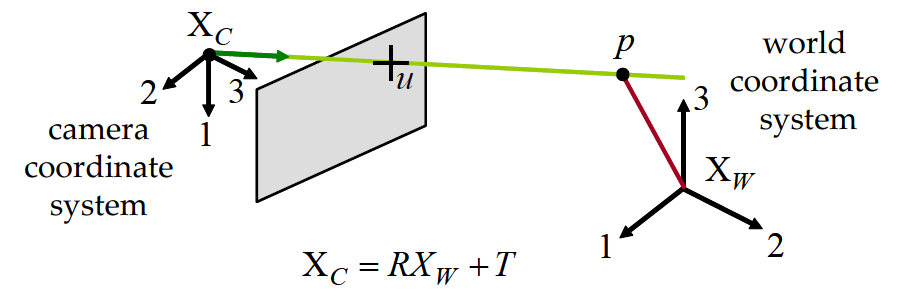
\includegraphics[width=0.8\textwidth]{figures/GeneralPinholeModel.PNG}
    \caption{General Pinhole Camera Model}
    \label{fig:PinholeCameraModel}
\end{figure}

\subsection{Creating a Point Cloud from the Depth Data}

This step is an intermediary one towards creating a mesh structure on which textures can be projected. A 3D point cloud is a set of data points in the third dimension, usually defined by $(X, Y, Z)$ coordinates.

The depth camera retrieves an image of 320x240 depth pixels. A point cloud can be created by using x, y values from 0 to the width and height of the depth image, respectively. The z value is simply equal to the depth, if the depth value is in a certain range(after it has been filtered). If the depth value is invalid, the current point is discarded and will not be rendered.

Further, the point cloud must be updated in real-time. Rendering is being done with OpenGL, and the previous can be accomplished by using simple hardware graphics shader programs and OpenGL's Vertex Buffer Objects(VBO). The OpenGL point cloud also has to be rotated, as it is upside down(unless the depth camera is positioned upside down).

In the following, I will include a subsection with information about the general rendering process, which is applied to render 3D objects with the programmable OpenGL pipeline. The process is similar, whether we wish to render a point cloud, or a 3D mesh, only the vertex attributes(position, color, texture coordinates, normals etc.) which are stored in the VBOs and the programmable shaders will change.

\subsubsection{Rendering}

The transformation pipeline(see figure \ref{fig:TransformationPipeline}) describes how the vertex information is transformed from raw data, to window coordinates that can be viewed on a screen. The raw vertices are first multiplied by the modelview matrix, which yields the transformed eye(view) coordinates. Then, we multiply the result by the projection matrix and obtain clip coordinates. All data outside the clipping space(frustum) is removed. Then, coordinates are divided by the $w$ value to yield normalized device coordinates  in the +/-1.0 range, for all axes. Finally, OpenGL internally maps the scene to a 2D plane by the viewport transformation matrix, based on the viewport parameters provided.

\begin{figure}[hbtp]
    \centering
    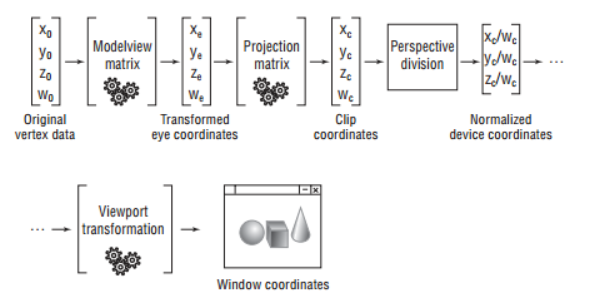
\includegraphics[width=0.8\textwidth]{figures/TransformationPipeline.PNG}
    \caption{Vertex Transformation Pipeline. Courtesy of \cite{superbible}}
    \label{fig:TransformationPipeline}
\end{figure}


In the following, I will briefly describe the 3D graphics pipeline, shown in figure \ref{fig:GraphicsPipeline}. It explains the stages required to process the vertices in order to obtain colored pixels and how vertex attributes can be programmed in the two shader stages(using the vertex and fragment processors).

\begin{figure}[hbtp]
    \centering
    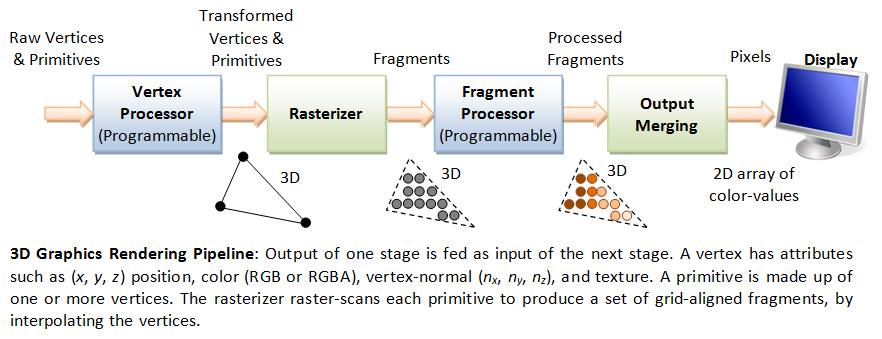
\includegraphics[width=0.8\textwidth]{figures/Graphics3D_Pipe.png}
    \caption{3D Graphics Pipeline}
    \label{fig:GraphicsPipeline}
\end{figure}

As we can see from the pipeline, the raw vertices are processed by a vertex processor which manipulates vertex related attributes, most generally, position. For example, a vertex shader(a program that runs on this processor) can be used to apply the modelview matrix to an input vertex. Next, the data is rasterized into fragments.
 
A fragment contains the data necessary to generate a single pixel's worth of a drawing primitive in the frame buffer(the frame buffer is a portion of memory that contains a bitmap that will be sent to the video display - it represents a complete frame of data): raster position, depth and, after the fragment shader stage, it also contains interpolated attributes such as color and texture coordinates as well as a stencil value, an alpha value and the window ID. Note that a fragment only corresponds to a pixel if antialiasing is turned off, otherwise there will be $K$ fragments for a pixel for $Kx$ level antialiasing.
As we can see from the above, the fragment shader receives fragments and processes them, computing color and texture coordinates. This shader can be programmed to color the geometry in any way desired. One can also apply textures and lighting at this stage. Finally, fragment shaders are also useful for visual debugging, as shader programs can usually not be debugged, since they run on the GPU hardware.\\

\subsubsection{Limitations}

Unfortunately, unless the point cloud is of sub-pixel density(which would also require a lot of processing power, due to the very large number of OpenGL primitives), it is easy to see that the target object is in fact made of discrete points(see figure \ref{fig:PointCloud}). This breaks immersion, especially after applying a texture to the object. Due to this, we must then proceed to the following step, triangulation of the points into a 3D mesh.

\begin{figure}[hbtp]
    \centering
    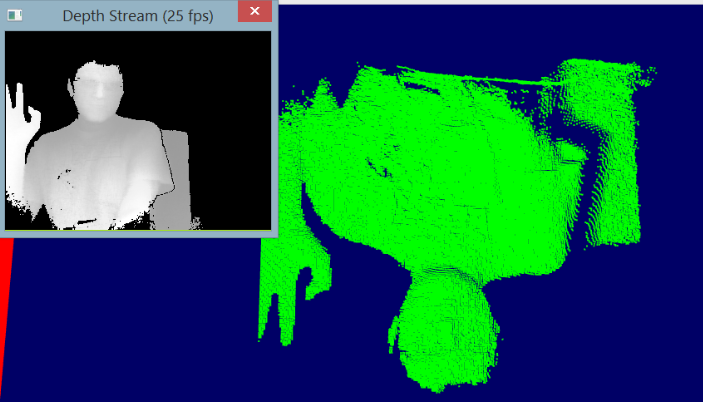
\includegraphics[width=0.8\textwidth]{figures/PointCloud.PNG}
    \caption{An example point cloud, corresponding to the depth stream, updated in real-time.}
    \label{fig:PointCloud}
\end{figure}

 However, before we proceed, we must also unproject the points to world coordinates(we just had pixel positions and depth values, but we need to obtain the coordinates in regular metric space, so that the distances between the points are correct). This operation requires knowledge about camera parameters, since we need to know the projection and view matrices, in order to unproject them:

$$point => Viewport^{-1} => Projection^{-1} => ModelView^{-1} => PointInWorldSpace$$



\subsection{Object Reconstruction by Mesh Triangulation}

There are several techniques for reconstructing a 3D mesh from a point cloud. An important aspect for our deformable display is that we only need a 2.5D correct mesh, similar to a terrain(see figure \ref{fig:PerspectiveTerrain}) or heightmap. 

\begin{figure}[hbtp]
    \centering
    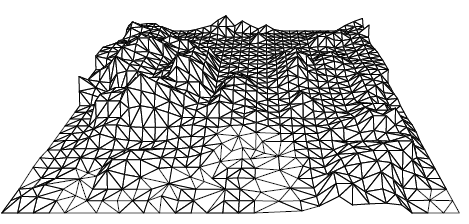
\includegraphics[width=0.4\textwidth]{figures/PerspectiveTerrain.PNG}
    \caption{Perspective View of Some Terrain. Courtesy of \cite[Chapter~9]{berg08}}
    \label{fig:PerspectiveTerrain}
\end{figure}



In order to obtain a full 3D model of an object, we would, anyway, need to rotate the depth camera around the object, or use multiple depth cameras, that look at the object from different angles. We always look from the front of the deformable display, as we would, down on a terrain, so such 3D detail is not needed. Therefore, the most straight-forward, naive approach, is to simply find any triangulation for the point cloud. In order to do this we can consider a grid of points, that can be connected either by using triangles or a triangle strip. The main idea of this method is also shown in figure \ref{fig:PolyhedralTerrain.PNG}, where a terrain is triangulated from some sample points.

\begin{figure}[hbtp]
    \centering
    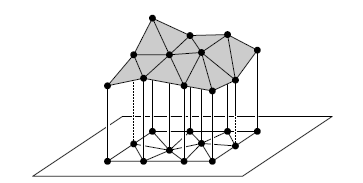
\includegraphics[width=0.4\textwidth]{figures/PolyhedralTerrain.PNG}
    \caption{Polyhedral(solid object with flat surfaces) Terrain. Smoothness will depend on point density. Courtesy of \cite[Chapter~9]{berg08}}
    \label{fig:PolyhedralTerrain.PNG}
\end{figure}

Although the naive approach has been implemented and used in this project, some more sophisticated alternatives will also be described and contrasted, as this approach was not the first one attempted.

\subsubsection{Connect a Grid of Points with a Triangle Strip}
\label{sec:TriangleStripTriangulation}
Since the depth data captured via a depth camera is ordered, the easiest way is to consider the point cloud as a grid of points. Then, one can connect the vertices together using triangle strips. Triangle strip representation is a method of drawing triangles that can save some of the memory bandwidth, by connecting a new triangle to an existing strip with each new point. This means, that, for example, if we want to draw two triangles, we only use 4 points, instead of 6, which we would normally need. An important thing to keep in mind is that triangle winding(the combination of order and direction in which the vertices are specified) is important. By default, OpenGL considers counterclockwise winding to represent front faces, and clockwise winding to represent backfaces. This enables the use of back-face culling for optimisation(we do not need to render triangles which are not visible), and are also important for normal calculation, and thus lighting. Although we are not concerned with lightning in this project, it is always good practice to keep the winding consistent. For more information about triangle strips and other OpenGL methods of drawing primtives please consult \cite[Chapter~3]{superbible}.

Coming back to the current problem, an internet article which explains how a triangle strip can be constructed from a grid of points is \cite{triangleStrip}. Figure \ref{fig:TriangleStrip} provides an overview, on how we can connect the vertices. Note that each point in the figure, numbered from 0-15 is a 3D vertex with coordinates $(x,y,z)$. 

\begin{figure}[hbtp]
    \centering
    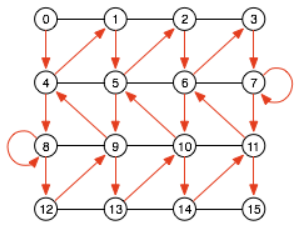
\includegraphics[width=0.6\textwidth]{figures/TriangleStripOrdering.PNG}
    \caption{Ordering of vertices in a triangle strip for a grid. Courtesy of \cite{triangleStrip}.}
    \label{fig:TriangleStrip}
\end{figure}

In this example, we can observe that on our path, we alternatively add 4 and subtract 3 for computing the next index, on the first row. On the next row, we still add 4, but subtract 5. The number 4 represents the number of vertices in the row or column, depending on how we advance($n + 1$ vertices, where n = number of divisions).
The numbers 3 and 5, correspond to $m = (n+1) + 1$ or $m = (n+1) - 1$ and represent changes between adjacent columns. The number alternates, depending on the order of traversal on that particular row.

This approach provides a decent reconstruction, for a 2.5D object using data from a single depth camera. Normals can also be computed after we have the geometry(at an additional computational cost), however, there is no need for lighting in our 3D scene, since we will be using textures as our final images. For improving the visual quality of the mesh, one could also look at more sophisticated methods of triangulation such as \textit{Delaunay Triangulation}, or use standard 3D reconstruction techniques, like the \textit{Marching Cubes} algorithm.

\subsubsection{Other Methods for 2.5D Triangulation}

The naive triangulation, by connecting the triangles without considering some measure of how natural it looks, may not provide the intuitively \textit{best-looking} results. If the triangulation is not acceptable, it can be improved with a technique such as \textbf{Delaunay Triangulation}(explained in detail in \cite[Chapter~9]{berg08}), where triangulations are ranked by comparing their smallest angle(small angles, result in \textit{skinniness}). The issue is shown in figure \ref{fig:MountainRidgeNarrowValley} where two triangulations of the same point set are shown. From the heights of the sample points, it seems as though the points were taken from a \textit{mountain ridge}. If an edge is flipped to obtain very small angles for our triangles, we get what looks as a \textit{narrow valley}(as you can see, the height value is now very small). The latter is a suboptimal triangulation and can be improved. Delaunay triangulation aims to find an optimal triangulation, given the fact that, for any set of points, there is a finite amount of possible triangulations.

However, for a dense set of points, such that obtained from the depth data, a naive triangle strip triangulation has provided adequate results - the deformation is clearly visible, both in the mesh and on the texture applied to the mesh. For this reason, Delaunay triangulation has not been attempted, although it may improve visual quality. It remains to be determined, as future work, if the computational cost involved is worth the possible increase in visual quality.

\begin{figure}[hbtp]
    \centering
    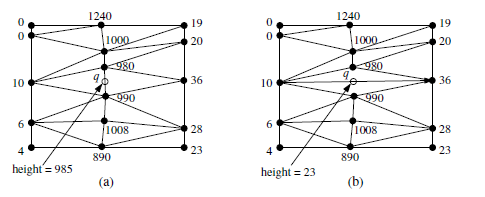
\includegraphics[width=0.4\textwidth]{figures/MountainRidgeNarrowValley.PNG}
    \caption{a)Mountain ridge; b) Narrow valley. Courtesy of \cite[Chapter~9]{berg08}}
    \label{fig:MountainRidgeNarrowValley}
\end{figure}


\subsubsection{Marching Cubes on GPU}

One of the classic computer algorithms for surface reconstruction is the \textit{Marching Cubes}  algorithm. An attempt was made to implement this algorithm. In order to run it on a GPU, one can use a \textit{geometry shader} or\textit{ histogram pyramids} with a regular vertex and fragment shader. The attempt consisted of porting an existing implementation of the geometry shader for fixed-pipeline OpenGL to modern OpenGL. Unfortunately, I did not get any geometry as output after running the algorithm, but there were also no errors. The problem is that I could not debug the shaders, since the tools I have tried did not work - some because of no support for modern OpenGL(3.0+) like \textit{glslDevil}, and others did not work on my laptop because it uses the \textit{nVidia Optimus} technology, as is the case for the \textit{nVidia nSight} debugging tool for \textit{Microsoft Visual Studio}. As this was taking too much time, I decided to go for a simpler approach, that should still prove appropriate for the real-time 3D reconstruction of the cloth, described in section \ref{sec:TriangleStripTriangulation}. Nevertheless I will briefly describe the algorithm in the following section, as well as how it can be implemented on a GPU. This may be useful to look into, as an extension to the current project, if a higher quality mesh is desired(this method works well for 3D objects in general, and is not restricted to 2.5D, as is the case for the currently used method).

\paragraph{The Marching Cubes Algorithm}\mbox{}\\

It was originally designed to create triangle models  from 3D medical data - usually volumetric data, using voxels for representation(voxels are similar to pixels, only they exist in 3D space and can be represented as a cube). The algorithm also needs each vertex of the dataset to have a scalar value, that usually represents a property of the underlying data set. An example of such a voxel set is shown in figure \ref{fig:VoxelSet}. This value will be used to construct an isosurface, by comparing where vertices of the voxel edges intersect the surface(given a constant user-defined threshold or isovalue).

\begin{figure}[hbtp]
    \centering
    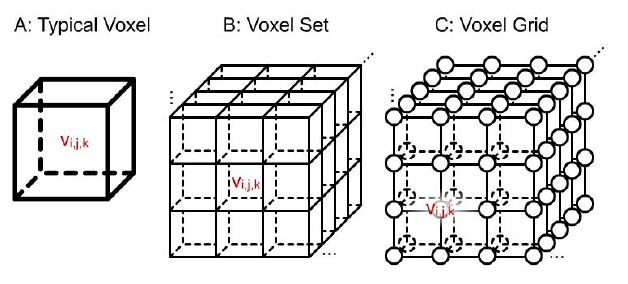
\includegraphics[width=0.4\textwidth]{figures/Voxels.PNG}
    \caption{Voxel data representation. Courtesy of \cite{navpreet2013}}
    \label{fig:VoxelSet}
\end{figure}


 The authors of the original paper on the topic state in \cite{william87} that two primary steps were used in their approach:
\begin{itemize}
\item Locating the surface corresponding to a user-specified value(isolevel) and creating triangles.
\item Calculating normals to the surface at each vertex of each triangle, in order to ensure a high quality image.
\end{itemize}

Since only the 3D mesh coordinates are required in order to capture the distortion of the cloth, the issue of calculating normals will not be described further, and we shall focus on the first part of the algorithm(although it should be mentioned that a fully shaded, reconstructed model could be useful for some calibration approaches, since, at the time of this writing there are no reconstruction libraries for the depth camera used in this project).

The algorithm uses a divide-and-conquer approach by using logical cubes of eight pixels to locate the surface. How the surface intersects every such cube needs to be determined. In order to do this, a value of one is assigned to a cube's vertex, if the data value at that vertex exceeds the value of the surface we are constructing(if the scalar value is above a threshold called the isolevel). These vertices are inside the surface. Conversely, a zero value is assigned to values below, and thus outside, the surface. The surface intersects the cube edges where one vertex is inside and the other outside.

Moreover, there are eight vertices in each cube and two states(inside and outside) so we have a total of $2^{8} = 256$ cases for intersection with such a cube. However, by eliminating symmetries, like complementary cases and rotational symmetry, the number of distinct cases of triangulation can be reduced to 14 patterns.

\begin{figure}[hbtp]
    \centering
    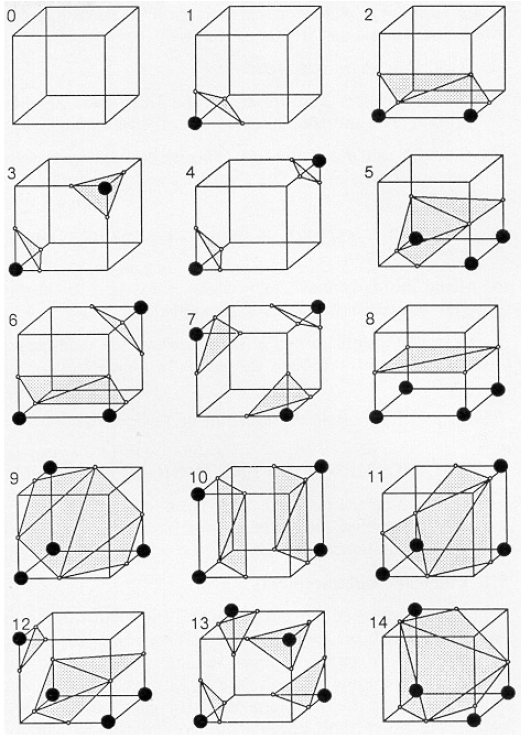
\includegraphics[width=0.4\textwidth]{figures/MarchingCubesTriagulationCases.PNG}
    \caption{Marching Cubes - The 14 Patterns of Triangulated Cubes. Courtesy of \cite{william87}}
    \label{fig:MarchingCubesTrianglatedCubes}
\end{figure}

As an example, the cube for pattern one in figure \ref{fig:MarchingCubesTrianglatedCubes} contains one  of the surface vertices(the lower-left vertex of the front face) and results in one triangle defined by three edge intersections. An eight bit index is created for each case, and it corresponds to the cube's vertex states(see figure \ref{fig:MarchingCubesLabeling}). This index points to an edge tables that retrieves all of the edge intersections for the given cube configuration. The triangles are calculated using linear interpolation of the scalar values along the vertices of the respective edges(to determine the exact location of the triangle vertices on the cube edges). As described in \cite{navpreet2013}, if $P1$ and $P2$ are the vertices of an intersected edge and $V1$ and $V2$ are the scalar values of each vertex, the intersection point $P$ is calculated as following:  
	$$P = P_{1} + (isovalue - V_{1})(P_{2} - P_{1}) / (V_{2} - V_{1})$$

\begin{figure}[hbtp]
    \centering
    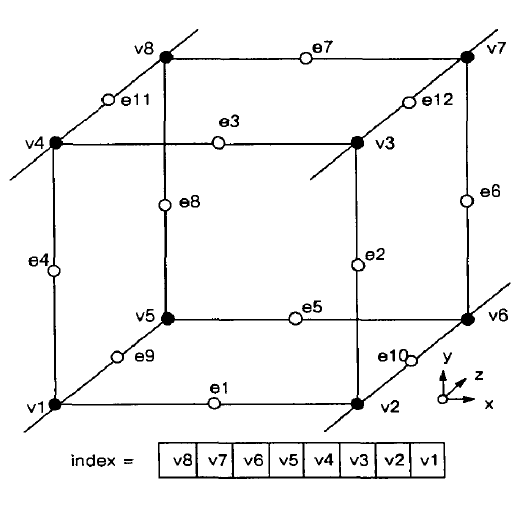
\includegraphics[width=0.4\textwidth]{figures/MarchingCubesNumbering.PNG}
    \caption{Marching Cubes - Cube Numbering. Courtesy of \cite{william87}}
    \label{fig:MarchingCubesLabeling}
\end{figure}

\paragraph{GPU Implementation}\mbox{}\\

\subparagraph{Geometry Shader}\mbox{}\\

Many aspects from a classical implementation of marching cubes can also be used for a GPU implementation. This is the case with the basic look-up tables used to store edges and triangles. A version of these tables used in several implementations is available in an on-line article(see \cite{bourke1994}), where the full source code is also available. Although, there is no version implemented in a programmable shader on the GPU available, an implementation using a geometry shader is described in another on-line article(see \cite{crassin2007}). A geometry shader is simply a shader program that can be used to manipulate geometry directly - it allows the GPU to create geometry. This shader takes a single primitive as input(e.g.: a vertex) and outputs zero or more primitives(e.g.: zero or more triangles). 
This implementation is based on \cite{bourke1994}, with the main marching cubes logic inside the geometry shader. However, this implementation also uses deprecated OpenGL functionality. The main idea is that data can be stored inside 2D and 3D textures and can then be passed to the geometry shader as uniforms:

\begin{verbatim}
//Volume data field texture
uniform sampler3D dataFieldTex;
//Edge table texture
uniform isampler2D edgeTableTex;
//Triangles table texture
uniform isampler2D triTableTex;
//Global iso level
uniform float isolevel;
//Marching cubes vertices decal
uniform vec3 vertDecals[8];
\end{verbatim}

In this code fragment  the $dataFieldTex$ contains the 3D voxel scalar field data, the $edgeTableTex$ contains which edges intersect the current cube index, and the $triTableTex$ contains all the triangle indices needed, corresponding to each case. Next, the cube index is calculated by comparing the value in the grid(retrieved from $dataFieldTex$) with the $isolevel$ uniform. The position is retrieved by adding to the current vertex(to move the vertex at the appropriate position in the cube), the value in $vertDecals$. This adds the required offset in the $x,y$ or $z$ directions by an amount of $cubeStep$, which is defined initially. Having the cube vertex positions and scalar values, the interpolated values can now be calculated, for each edge. The final triangle vertices are retrieved by using the indices in $triTableTex$, for the previously computed interpolated values.

\subparagraph{Histogram Pyramids}\mbox{}\\

Another approach is to use histogram pyramids, as described in \cite{dyken2007}. The authors state that their algorithm outperforms the known geometry shader approaches and it does not take much more effort to implement. The hierarchical data structured called the \textit{HistoPyramid}, used for data expansion and compaction of 2D textures, is the focus of the previously mentioned paper. The term texel was used to denote single data elements, and the 3D array of voxels has been mapped to a 2D domain.


\paragraph{Implicit Surface Generation}\mbox{}\\

As stated before, in order to use the marching cubes algorithm, one also needs to obtain a scalar value at each point in the data set, and, since we only have a point cloud, a function is needed to provide this - such a dataset is called an implicit surface. These functions were not a focus for this project, as the marching cubes algorithms was not successfully run on datasets that already represented implicit surfaces. However, in \cite{navpreet2013} the Hermite Radial Basis Function(HRBF) is mentioned as a workable method, please consult this resource for more information on the topic. Another function that can determine the scalar field is the Newtonian gravity field equation, please consult \cite{max2013} for further information.

\subsubsection{Greedy Triangulation}
\subsubsection{Kinect Fusion and Kinfu}

\subsection{Projective Texture Mapping}

An article by NVIDIA which also references \cite{segal92}, describes projective texture mapping and how it can be implemented using OpenGL (see \cite{cassNvidia}). A short summary of this is presented below.

For projective texture mapping we need to use homogeneous texture coordinates. For example, for a projective 2D texture we have the coordinates (s,t,q) where the interpolated homogeneous coordinate is projected to a real 2D texture coordinate by dividing both s and t by q to obtain, (s/q, t/q). The homogeneous texture coordinates have to be assigned per-vertex. The final step implies a range mapping with [0,1] for each coordinate (using a scale and bias, so that the texture coordinates change from [-1,1] to [0,1]). In figure \ref{fig:VirtualProjectorPipeline} the transforms that are applied to a vertex position in order to compute projective texture coordinates are displayed.

\begin{figure}[hbtp]
    \centering
    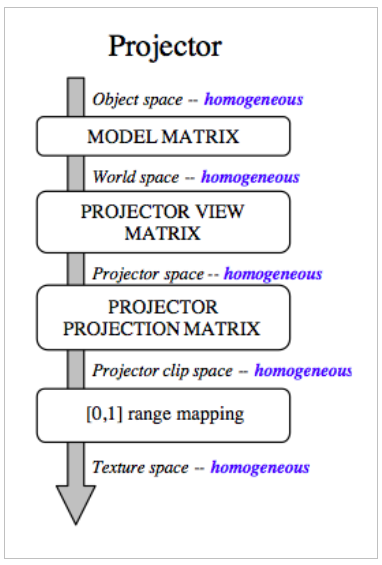
\includegraphics[width=0.4\textwidth]{figures/VirtualProjectorPipeline.PNG}
    \caption{Virtual Projector Transformation Pipeline. Courtesy of \cite{cassNvidia}}
    \label{fig:VirtualProjectorPipeline}
\end{figure}

The vertex position in object and eye space is used to generate the texture coordinate. In OpenGL this can be accomplished with the \textit{texgen} facility (generates texture coordinates from vector attributes). In the \textit{object} and \textit{eye linear} modes, the texture coordinate is computed by solving a plane equation at the vertex position. Evaluating a plane equation is equivalent to a 4-component dot product, so the texgen planes form a 4x4 matrix, $T$:

\begin{figure}[hbtp]
    \centering
    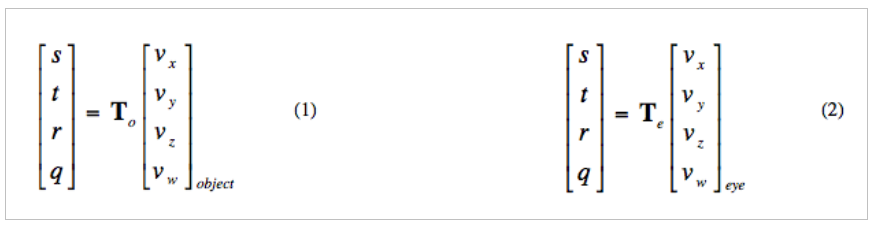
\includegraphics[width=1.0\textwidth]{figures/PTMCoordinates.PNG}
    \caption{Projective Texture Coordinates from a 4x4 matrix and the vertices in object or eye space. Courtesy of \cite{cassNvidia}}
    \label{fig:ProjectiveTextureMapping}
\end{figure}

where $s, t, r, q$ are the texture coordinates, $v$ are the vertices in \textit{eye} or \textit{object} space and $T$ is the texgen matrix in eye or object space.

\subsubsection{Object Linear Texgen}

The object linear texgen can be represented as shown in figure \ref{fig:ObjectLinearTexgen}, where the first matrix is the scale-bias matrix, $M$ is the model matrix (in our case this should be the model matrix of the deformable display), $V_{p}$ is the view matrix for the projector and $P_{p}$ is the projector's projection matrix.

\begin{figure}[hbtp]
    \centering
    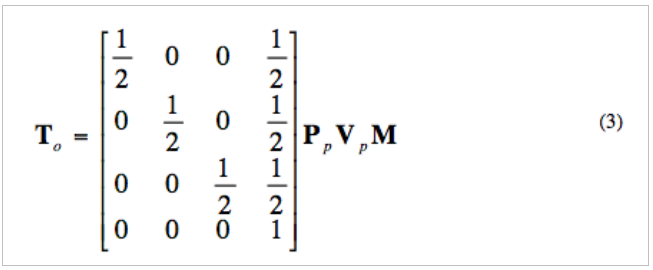
\includegraphics[width=0.6\textwidth]{figures/ObjectLinearTexgen.PNG}
    \caption{Object Linear Texgen. Courtesy of \cite{cassNvidia}}
    \label{fig:ObjectLinearTexgen}
\end{figure}

\subsubsection{Eye Linear Texgen}

The object linear texgen can be represented as shown in figure \ref{fig:EyeLinearTexgen}, where the same notations are used as in the previous section, but instead of multiplying with the model matrix $M$ in the end, we multiply with $V^{-1}_{e}$ which is the inverse of the eye(or camera) view matrix.

\begin{figure}[hbtp]
    \centering
    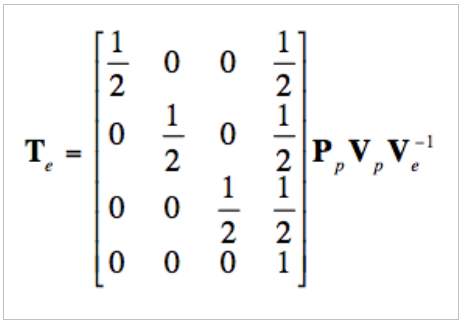
\includegraphics[width=0.4\textwidth]{figures/EyeLinearTexgen.PNG}
    \caption{Eye Linear Texgen. Courtesy of \cite{cassNvidia}}
    \label{fig:EyeLinearTexgen}
\end{figure}

\subsection{Capturing Dynamic Contents}

\section{Prototype Implementation}
\section{Conclusions}
\section{Future Work}

\newpage
\bibliography{bibliography}
\bibliographystyle{plain}

\end{document}
